\section{Problem 3}

\subsection{Question}
\vspace*{10pt}
Determine if the friendship paradox holds for your Twitter account.
Since Twitter is a directed graph, use \enquote{followers} as value you measure 
$($i.e., \enquote{do your followers have more followers than you?}$)$.\\
\\
Generate the same graph as in question \#1, and calcuate the same 
mean, standard deviation, and median values.\\
\\
For the Twitter 1.1 API to help gather this data, see:
\\
\url{https://dev.twitter.com/docs/api/1.1/get/followers/list}
\\
If you do not have followers on Twitter (or don't have more than 50),
then use my twitter account \enquote{phonedude\_mln}.

\subsection{Answer}
Fortunately, {\it linkedIn} provides information about connections (people) through an API\cite{linkedin}. I have written a Python program,
{\it qet\_linkedin}, that requests\cite{oauth2} data from {\it linkedIn} and saves the output into linkedin\_count.
\vspace{3mm}
\lstinputlisting[language=Python, caption={get\_linkedin.py}, label=listing:get_linkedin]{q3/get_linkedin.py}
\clearpage
\vspace{2mm}
I would like indicate here that the API that LinkedIn provides returns no more than 500 connection. In other words, if I have someone in my connection has more than 500 connections. LinkedIn will give me this person has 500+.

The {\tt linkedin\_count} file was ordered in place with the Unix command in Listing \ref{listing:sort2}. 
\vspace{2mm}
\begin{lstlisting}[language=Bash,caption={Sort command},label=listing:sort2]
Naina Sai Tipparti@DESKTOP-2FU7AJC ~/a4/q3 cat linkedin_count | sort -g -o linkedin_count
\end{lstlisting}
\vspace{2mm}
This file was then processed by the R script shown in Listing \ref{listing:linkedin_graphr} to produce the graph in Figure \ref{fig:linkedin_graph}

\lstinputlisting[language=R, caption={Graph Creation Script for LinkedIn}, label=listing:linkedin_graphr]{q3/plot_linkedin.R}
\clearpage
\vspace*{2mm}
\begin{table}
\centering
\begin{tabular}{ l l }
\hline
\textbf{Mean} & 156.875 \\
\textbf{Median} & 95 \\
\textbf{Std Dev} & 154.6315
\\
\hline
\end{tabular}
\caption{Statistics on the count of Naina Sai Tipparti's LinkedIn, values straight from R}
\label{tab:q3stats}
\end{table}
\begin{figure}[h!]
\centering
\fbox{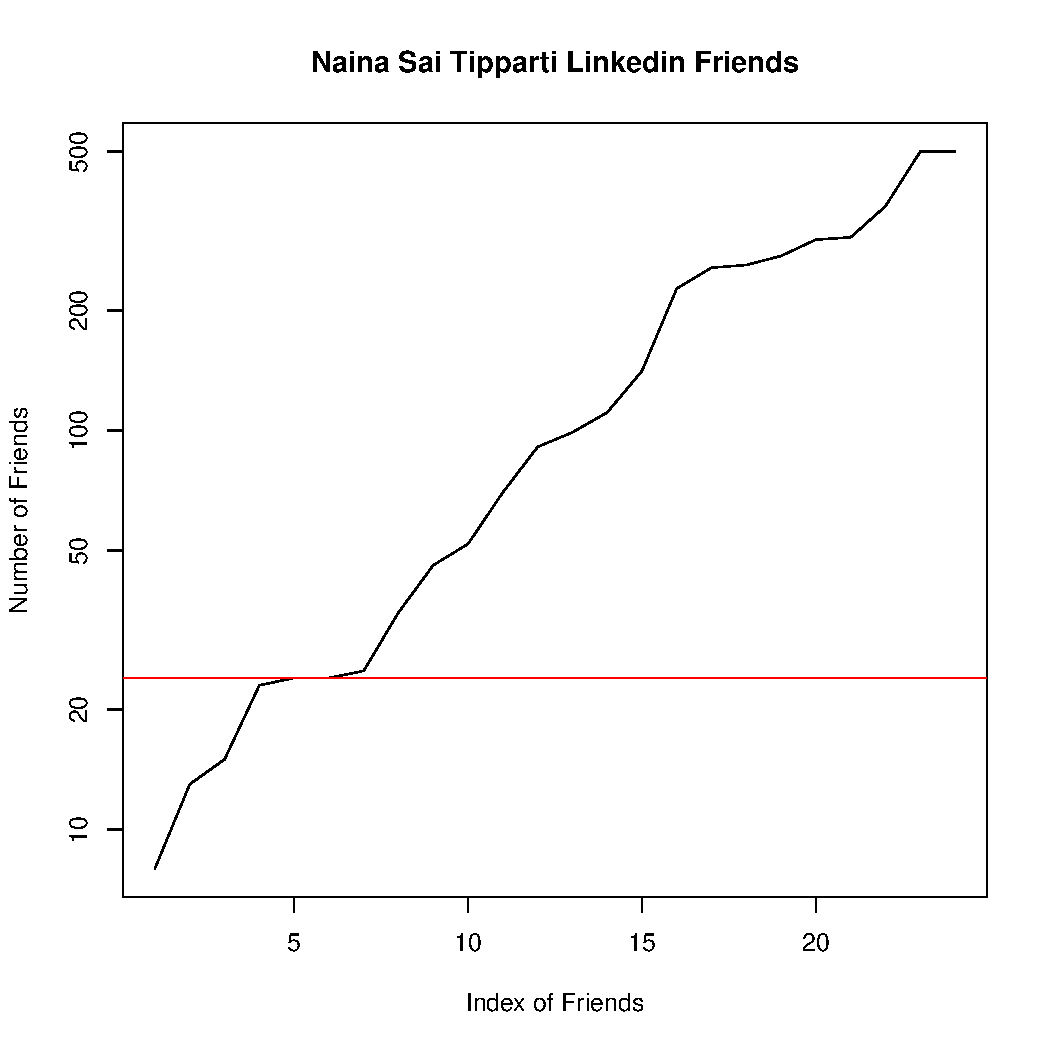
\includegraphics[scale=0.75]{q3/linkedin_plot.pdf}}
\caption{The Friendship Graph for LinkedIn}
\label{fig:linkedin_graph}
\end{figure}
I have number of connections which is a way less than the mean, but we can not conclude from the above statistics that the friendship paradox holds for My LinkedIn account since must of my connections have connections greater the mean. 